\documentclass[11pt,compress,t,notes=noshow, xcolor=table]{beamer}
\usepackage[]{graphicx}\usepackage[]{color}
% maxwidth is the original width if it is less than linewidth
% otherwise use linewidth (to make sure the graphics do not exceed the margin)
\makeatletter
\def\maxwidth{ %
  \ifdim\Gin@nat@width>\linewidth
    \linewidth
  \else
    \Gin@nat@width
  \fi
}
\makeatother

\definecolor{fgcolor}{rgb}{0.345, 0.345, 0.345}
\newcommand{\hlnum}[1]{\textcolor[rgb]{0.686,0.059,0.569}{#1}}%
\newcommand{\hlstr}[1]{\textcolor[rgb]{0.192,0.494,0.8}{#1}}%
\newcommand{\hlcom}[1]{\textcolor[rgb]{0.678,0.584,0.686}{\textit{#1}}}%
\newcommand{\hlopt}[1]{\textcolor[rgb]{0,0,0}{#1}}%
\newcommand{\hlstd}[1]{\textcolor[rgb]{0.345,0.345,0.345}{#1}}%
\newcommand{\hlkwa}[1]{\textcolor[rgb]{0.161,0.373,0.58}{\textbf{#1}}}%
\newcommand{\hlkwb}[1]{\textcolor[rgb]{0.69,0.353,0.396}{#1}}%
\newcommand{\hlkwc}[1]{\textcolor[rgb]{0.333,0.667,0.333}{#1}}%
\newcommand{\hlkwd}[1]{\textcolor[rgb]{0.737,0.353,0.396}{\textbf{#1}}}%
\let\hlipl\hlkwb

\usepackage{framed}
\makeatletter
\newenvironment{kframe}{%
 \def\at@end@of@kframe{}%
 \ifinner\ifhmode%
  \def\at@end@of@kframe{\end{minipage}}%
  \begin{minipage}{\columnwidth}%
 \fi\fi%
 \def\FrameCommand##1{\hskip\@totalleftmargin \hskip-\fboxsep
 \colorbox{shadecolor}{##1}\hskip-\fboxsep
     % There is no \\@totalrightmargin, so:
     \hskip-\linewidth \hskip-\@totalleftmargin \hskip\columnwidth}%
 \MakeFramed {\advance\hsize-\width
   \@totalleftmargin\z@ \linewidth\hsize
   \@setminipage}}%
 {\par\unskip\endMakeFramed%
 \at@end@of@kframe}
\makeatother

\definecolor{shadecolor}{rgb}{.97, .97, .97}
\definecolor{messagecolor}{rgb}{0, 0, 0}
\definecolor{warningcolor}{rgb}{1, 0, 1}
\definecolor{errorcolor}{rgb}{1, 0, 0}
\newenvironment{knitrout}{}{} % an empty environment to be redefined in TeX

\usepackage{alltt}
\newcommand{\SweaveOpts}[1]{}  % do not interfere with LaTeX
\newcommand{\SweaveInput}[1]{} % because they are not real TeX commands
\newcommand{\Sexpr}[1]{}       % will only be parsed by R
\newcommand{\xmark}{\ding{55}}%


\usepackage[english]{babel}
\usepackage[utf8]{inputenc}

\usepackage{dsfont}
\usepackage{verbatim}
\usepackage{amsmath}
\usepackage{amsfonts}
\usepackage{amssymb}
\usepackage{bm}
\usepackage{csquotes}
\usepackage{multirow}
\usepackage{longtable}
\usepackage{booktabs}
\usepackage{enumerate}
\usepackage[absolute,overlay]{textpos}
\usepackage{psfrag}
\usepackage{algorithm}
\usepackage{algpseudocode}
\usepackage{eqnarray}
\usepackage{arydshln}
\usepackage{tabularx}
\usepackage{placeins}
\usepackage{tikz}
\usepackage{setspace}
\usepackage{colortbl}
\usepackage{mathtools}
\usepackage{wrapfig}
\usepackage{bm}
\usepackage{amsmath}
\usepackage{pifont}

\usetikzlibrary{shapes,arrows,automata,positioning,calc,chains,trees, shadows}
\tikzset{
  %Define standard arrow tip
  >=stealth',
  %Define style for boxes
  punkt/.style={
    rectangle,
    rounded corners,
    draw=black, very thick,
    text width=6.5em,
    minimum height=2em,
    text centered},
  % Define arrow style
  pil/.style={
    ->,
    thick,
    shorten <=2pt,
    shorten >=2pt,}
}

\usepackage{subfig}

% Defines macros and environments
\usepackage{../../style/lmu-lecture}


\let\code=\texttt
\let\proglang=\textsf

\setkeys{Gin}{width=0.9\textwidth}

\setbeamertemplate{frametitle}{\expandafter\uppercase\expandafter\insertframetitle}

\usepackage{bbm}
% basic latex stuff
\newcommand{\pkg}[1]{{\fontseries{b}\selectfont #1}} %fontstyle for R packages
\newcommand{\lz}{\vspace{0.5cm}} %vertical space
\newcommand{\dlz}{\vspace{1cm}} %double vertical space
\newcommand{\oneliner}[1] % Oneliner for important statements
{\begin{block}{}\begin{center}\begin{Large}#1\end{Large}\end{center}\end{block}}


%new environments
\newenvironment{vbframe}  %frame with breaks and verbatim
{
 \begin{frame}[containsverbatim,allowframebreaks]
}
{
\end{frame}
}

\newenvironment{vframe}  %frame with verbatim without breaks (to avoid numbering one slided frames)
{
 \begin{frame}[containsverbatim]
}
{
\end{frame}
}

\newenvironment{blocki}[1]   % itemize block
{
 \begin{block}{#1}\begin{itemize}
}
{
\end{itemize}\end{block}
}

\newenvironment{fragileframe}[2]{  %fragile frame with framebreaks
\begin{frame}[allowframebreaks, fragile, environment = fragileframe]
\frametitle{#1}
#2}
{\end{frame}}


\newcommand{\myframe}[2]{  %short for frame with framebreaks
\begin{frame}[allowframebreaks]
\frametitle{#1}
#2
\end{frame}}

\newcommand{\remark}[1]{
  \textbf{Remark:} #1
}

\newcommand{\citebutton}[2]{%
\NoCaseChange{\resizebox{!}{9pt}{\protect\beamergotobutton{\href{#2}{#1}}}}%
}



\newenvironment{deleteframe}
{
\begingroup
\usebackgroundtemplate{\includegraphics[width=\paperwidth,height=\paperheight]{../style/color/red.png}}
 \begin{frame}
}
{
\end{frame}
\endgroup
}
\newenvironment{simplifyframe}
{
\begingroup
\usebackgroundtemplate{\includegraphics[width=\paperwidth,height=\paperheight]{../style/color/yellow.png}}
 \begin{frame}
}
{
\end{frame}
\endgroup
}\newenvironment{draftframe}
{
\begingroup
\usebackgroundtemplate{\includegraphics[width=\paperwidth,height=\paperheight]{../style/color/green.jpg}}
 \begin{frame}
}
{
\end{frame}
\endgroup
}
% https://tex.stackexchange.com/a/261480: textcolor that works in mathmode
\makeatletter
\renewcommand*{\@textcolor}[3]{%
  \protect\leavevmode
  \begingroup
    \color#1{#2}#3%
  \endgroup
}
\makeatother





% math spaces
\ifdefined\N                                                                
\renewcommand{\N}{\mathds{N}} % N, naturals
\else \newcommand{\N}{\mathds{N}} \fi 
\newcommand{\Z}{\mathds{Z}} % Z, integers
\newcommand{\Q}{\mathds{Q}} % Q, rationals
\newcommand{\R}{\mathds{R}} % R, reals
\ifdefined\C 
  \renewcommand{\C}{\mathds{C}} % C, complex
\else \newcommand{\C}{\mathds{C}} \fi
\newcommand{\continuous}{\mathcal{C}} % C, space of continuous functions
\newcommand{\M}{\mathcal{M}} % machine numbers
\newcommand{\epsm}{\epsilon_m} % maximum error

% counting / finite sets
\newcommand{\setzo}{\{0, 1\}} % set 0, 1
\newcommand{\setmp}{\{-1, +1\}} % set -1, 1
\newcommand{\unitint}{[0, 1]} % unit interval

% basic math stuff
\newcommand{\xt}{\tilde x} % x tilde
\newcommand{\argmax}{\operatorname{arg\,max}} % argmax
\newcommand{\argmin}{\operatorname{arg\,min}} % argmin
\newcommand{\argminlim}{\mathop{\mathrm{arg\,min}}\limits} % argmax with limits
\newcommand{\argmaxlim}{\mathop{\mathrm{arg\,max}}\limits} % argmin with limits  
\newcommand{\sign}{\operatorname{sign}} % sign, signum
\newcommand{\I}{\mathbb{I}} % I, indicator
\newcommand{\order}{\mathcal{O}} % O, order
\newcommand{\pd}[2]{\frac{\partial{#1}}{\partial #2}} % partial derivative
\newcommand{\floorlr}[1]{\left\lfloor #1 \right\rfloor} % floor
\newcommand{\ceillr}[1]{\left\lceil #1 \right\rceil} % ceiling

% sums and products
\newcommand{\sumin}{\sum\limits_{i=1}^n} % summation from i=1 to n
\newcommand{\sumim}{\sum\limits_{i=1}^m} % summation from i=1 to m
\newcommand{\sumjn}{\sum\limits_{j=1}^n} % summation from j=1 to p
\newcommand{\sumjp}{\sum\limits_{j=1}^p} % summation from j=1 to p
\newcommand{\sumik}{\sum\limits_{i=1}^k} % summation from i=1 to k
\newcommand{\sumkg}{\sum\limits_{k=1}^g} % summation from k=1 to g
\newcommand{\sumjg}{\sum\limits_{j=1}^g} % summation from j=1 to g
\newcommand{\meanin}{\frac{1}{n} \sum\limits_{i=1}^n} % mean from i=1 to n
\newcommand{\meanim}{\frac{1}{m} \sum\limits_{i=1}^m} % mean from i=1 to n
\newcommand{\meankg}{\frac{1}{g} \sum\limits_{k=1}^g} % mean from k=1 to g
\newcommand{\prodin}{\prod\limits_{i=1}^n} % product from i=1 to n
\newcommand{\prodkg}{\prod\limits_{k=1}^g} % product from k=1 to g
\newcommand{\prodjp}{\prod\limits_{j=1}^p} % product from j=1 to p

% linear algebra
\newcommand{\one}{\boldsymbol{1}} % 1, unitvector
\newcommand{\zero}{\mathbf{0}} % 0-vector
\newcommand{\id}{\boldsymbol{I}} % I, identity
\newcommand{\diag}{\operatorname{diag}} % diag, diagonal
\newcommand{\trace}{\operatorname{tr}} % tr, trace
\newcommand{\spn}{\operatorname{span}} % span
\newcommand{\scp}[2]{\left\langle #1, #2 \right\rangle} % <.,.>, scalarproduct
\newcommand{\mat}[1]{\begin{pmatrix} #1 \end{pmatrix}} % short pmatrix command
\newcommand{\Amat}{\mathbf{A}} % matrix A
\newcommand{\Deltab}{\mathbf{\Delta}} % error term for vectors

% basic probability + stats
\renewcommand{\P}{\mathds{P}} % P, probability
\newcommand{\E}{\mathds{E}} % E, expectation
\newcommand{\var}{\mathsf{Var}} % Var, variance
\newcommand{\cov}{\mathsf{Cov}} % Cov, covariance
\newcommand{\corr}{\mathsf{Corr}} % Corr, correlation
\newcommand{\normal}{\mathcal{N}} % N of the normal distribution
\newcommand{\iid}{\overset{i.i.d}{\sim}} % dist with i.i.d superscript
\newcommand{\distas}[1]{\overset{#1}{\sim}} % ... is distributed as ...

% machine learning
\newcommand{\Xspace}{\mathcal{X}} % X, input space
\newcommand{\Yspace}{\mathcal{Y}} % Y, output space
\newcommand{\nset}{\{1, \ldots, n\}} % set from 1 to n
\newcommand{\pset}{\{1, \ldots, p\}} % set from 1 to p
\newcommand{\gset}{\{1, \ldots, g\}} % set from 1 to g
\newcommand{\Pxy}{\mathbb{P}_{xy}} % P_xy
\newcommand{\Exy}{\mathbb{E}_{xy}} % E_xy: Expectation over random variables xy
\newcommand{\xv}{\mathbf{x}} % vector x (bold)
\newcommand{\xtil}{\tilde{\mathbf{x}}} % vector x-tilde (bold)
\newcommand{\yv}{\mathbf{y}} % vector y (bold)
\newcommand{\xy}{(\xv, y)} % observation (x, y)
\newcommand{\xvec}{\left(x_1, \ldots, x_p\right)^\top} % (x1, ..., xp) 
\newcommand{\Xmat}{\mathbf{X}} % Design matrix
\newcommand{\allDatasets}{\mathds{D}} % The set of all datasets
\newcommand{\allDatasetsn}{\mathds{D}_n}  % The set of all datasets of size n 
\newcommand{\D}{\mathcal{D}} % D, data
\newcommand{\Dn}{\D_n} % D_n, data of size n
\newcommand{\Dtrain}{\mathcal{D}_{\text{train}}} % D_train, training set
\newcommand{\Dtest}{\mathcal{D}_{\text{test}}} % D_test, test set
\newcommand{\xyi}[1][i]{\left(\xv^{(#1)}, y^{(#1)}\right)} % (x^i, y^i), i-th observation
\newcommand{\Dset}{\left( \xyi[1], \ldots, \xyi[n]\right)} % {(x1,y1)), ..., (xn,yn)}, data
\newcommand{\defAllDatasetsn}{(\Xspace \times \Yspace)^n} % Def. of the set of all datasets of size n 
\newcommand{\defAllDatasets}{\bigcup_{n \in \N}(\Xspace \times \Yspace)^n} % Def. of the set of all datasets 
\newcommand{\xdat}{\left\{ \xv^{(1)}, \ldots, \xv^{(n)}\right\}} % {x1, ..., xn}, input data
\newcommand{\yvec}{\left(y^{(1)}, \hdots, y^{(n)}\right)^\top} % (y1, ..., yn), vector of outcomes
\renewcommand{\xi}[1][i]{\xv^{(#1)}} % x^i, i-th observed value of x
\newcommand{\yi}[1][i]{y^{(#1)}} % y^i, i-th observed value of y 
\newcommand{\xivec}{\left(x^{(i)}_1, \ldots, x^{(i)}_p\right)^\top} % (x1^i, ..., xp^i), i-th observation vector
\newcommand{\xj}{\xv_j} % x_j, j-th feature
\newcommand{\xjvec}{\left(x^{(1)}_j, \ldots, x^{(n)}_j\right)^\top} % (x^1_j, ..., x^n_j), j-th feature vector
\newcommand{\phiv}{\mathbf{\phi}} % Basis transformation function phi
\newcommand{\phixi}{\mathbf{\phi}^{(i)}} % Basis transformation of xi: phi^i := phi(xi)

%%%%%% ml - models general
\newcommand{\lamv}{\bm{\lambda}} % lambda vector, hyperconfiguration vector
\newcommand{\Lam}{\bm{\Lambda}}	 % Lambda, space of all hpos
% Inducer / Inducing algorithm
\newcommand{\preimageInducer}{\left(\defAllDatasets\right)\times\Lam} % Set of all datasets times the hyperparameter space
\newcommand{\preimageInducerShort}{\allDatasets\times\Lam} % Set of all datasets times the hyperparameter space
% Inducer / Inducing algorithm
\newcommand{\ind}{\mathcal{I}} % Inducer, inducing algorithm, learning algorithm 

% continuous prediction function f
\newcommand{\ftrue}{f_{\text{true}}}  % True underlying function (if a statistical model is assumed)
\newcommand{\ftruex}{\ftrue(\xv)} % True underlying function (if a statistical model is assumed)
\newcommand{\fx}{f(\xv)} % f(x), continuous prediction function
\newcommand{\fdomains}{f: \Xspace \rightarrow \R^g} % f with domain and co-domain
\newcommand{\Hspace}{\mathcal{H}} % hypothesis space where f is from
\newcommand{\fbayes}{f^{\ast}} % Bayes-optimal model
\newcommand{\fxbayes}{f^{\ast}(\xv)} % Bayes-optimal model
\newcommand{\fkx}[1][k]{f_{#1}(\xv)} % f_j(x), discriminant component function
\newcommand{\fh}{\hat{f}} % f hat, estimated prediction function
\newcommand{\fxh}{\fh(\xv)} % fhat(x)
\newcommand{\fxt}{f(\xv ~|~ \thetab)} % f(x | theta)
\newcommand{\fxi}{f\left(\xv^{(i)}\right)} % f(x^(i))
\newcommand{\fxih}{\hat{f}\left(\xv^{(i)}\right)} % f(x^(i))
\newcommand{\fxit}{f\left(\xv^{(i)} ~|~ \thetab\right)} % f(x^(i) | theta)
\newcommand{\fhD}{\fh_{\D}} % fhat_D, estimate of f based on D
\newcommand{\fhDtrain}{\fh_{\Dtrain}} % fhat_Dtrain, estimate of f based on D
\newcommand{\fhDnlam}{\fh_{\Dn, \lamv}} %model learned on Dn with hp lambda
\newcommand{\fhDlam}{\fh_{\D, \lamv}} %model learned on D with hp lambda
\newcommand{\fhDnlams}{\fh_{\Dn, \lamv^\ast}} %model learned on Dn with optimal hp lambda 
\newcommand{\fhDlams}{\fh_{\D, \lamv^\ast}} %model learned on D with optimal hp lambda 

% discrete prediction function h
\newcommand{\hx}{h(\xv)} % h(x), discrete prediction function
\newcommand{\hh}{\hat{h}} % h hat
\newcommand{\hxh}{\hat{h}(\xv)} % hhat(x)
\newcommand{\hxt}{h(\xv | \thetab)} % h(x | theta)
\newcommand{\hxi}{h\left(\xi\right)} % h(x^(i))
\newcommand{\hxit}{h\left(\xi ~|~ \thetab\right)} % h(x^(i) | theta)
\newcommand{\hbayes}{h^{\ast}} % Bayes-optimal classification model
\newcommand{\hxbayes}{h^{\ast}(\xv)} % Bayes-optimal classification model

% yhat
\newcommand{\yh}{\hat{y}} % yhat for prediction of target
\newcommand{\yih}{\hat{y}^{(i)}} % yhat^(i) for prediction of ith targiet
\newcommand{\resi}{\yi- \yih}

% theta
\newcommand{\thetah}{\hat{\theta}} % theta hat
\newcommand{\thetab}{\bm{\theta}} % theta vector
\newcommand{\thetabh}{\bm{\hat\theta}} % theta vector hat
\newcommand{\thetat}[1][t]{\thetab^{[#1]}} % theta^[t] in optimization
\newcommand{\thetatn}[1][t]{\thetab^{[#1 +1]}} % theta^[t+1] in optimization
\newcommand{\thetahDnlam}{\thetabh_{\Dn, \lamv}} %theta learned on Dn with hp lambda
\newcommand{\thetahDlam}{\thetabh_{\D, \lamv}} %theta learned on D with hp lambda
\newcommand{\mint}{\min_{\thetab \in \Theta}} % min problem theta
\newcommand{\argmint}{\argmin_{\thetab \in \Theta}} % argmin theta

% densities + probabilities
% pdf of x 
\newcommand{\pdf}{p} % p
\newcommand{\pdfx}{p(\xv)} % p(x)
\newcommand{\pixt}{\pi(\xv~|~ \thetab)} % pi(x|theta), pdf of x given theta
\newcommand{\pixit}{\pi\left(\xi ~|~ \thetab\right)} % pi(x^i|theta), pdf of x given theta
\newcommand{\pixii}{\pi\left(\xi\right)} % pi(x^i), pdf of i-th x 

% pdf of (x, y)
\newcommand{\pdfxy}{p(\xv,y)} % p(x, y)
\newcommand{\pdfxyt}{p(\xv, y ~|~ \thetab)} % p(x, y | theta)
\newcommand{\pdfxyit}{p\left(\xi, \yi ~|~ \thetab\right)} % p(x^(i), y^(i) | theta)

% pdf of x given y
\newcommand{\pdfxyk}[1][k]{p(\xv | y= #1)} % p(x | y = k)
\newcommand{\lpdfxyk}[1][k]{\log p(\xv | y= #1)} % log p(x | y = k)
\newcommand{\pdfxiyk}[1][k]{p\left(\xi | y= #1 \right)} % p(x^i | y = k)

% prior probabilities
\newcommand{\pik}[1][k]{\pi_{#1}} % pi_k, prior
\newcommand{\lpik}[1][k]{\log \pi_{#1}} % log pi_k, log of the prior
\newcommand{\pit}{\pi(\thetab)} % Prior probability of parameter theta

% posterior probabilities
\newcommand{\post}{\P(y = 1 ~|~ \xv)} % P(y = 1 | x), post. prob for y=1
\newcommand{\postk}[1][k]{\P(y = #1 ~|~ \xv)} % P(y = k | y), post. prob for y=k
\newcommand{\pidomains}{\pi: \Xspace \rightarrow \unitint} % pi with domain and co-domain
\newcommand{\pibayes}{\pi^{\ast}} % Bayes-optimal classification model
\newcommand{\pixbayes}{\pi^{\ast}(\xv)} % Bayes-optimal classification model
\newcommand{\pix}{\pi(\xv)} % pi(x), P(y = 1 | x)
\newcommand{\pikx}[1][k]{\pi_{#1}(\xv)} % pi_k(x), P(y = k | x)
\newcommand{\pikxt}[1][k]{\pi_{#1}(\xv ~|~ \thetab)} % pi_k(x | theta), P(y = k | x, theta)
\newcommand{\pixh}{\hat \pi(\xv)} % pi(x) hat, P(y = 1 | x) hat
\newcommand{\pikxh}[1][k]{\hat \pi_{#1}(\xv)} % pi_k(x) hat, P(y = k | x) hat
\newcommand{\pixih}{\hat \pi(\xi)} % pi(x^(i)) with hat
\newcommand{\pikxih}[1][k]{\hat \pi_{#1}(\xi)} % pi_k(x^(i)) with hat
\newcommand{\pdfygxt}{p(y ~|~\xv, \thetab)} % p(y | x, theta)
\newcommand{\pdfyigxit}{p\left(\yi ~|~\xi, \thetab\right)} % p(y^i |x^i, theta)
\newcommand{\lpdfygxt}{\log \pdfygxt } % log p(y | x, theta)
\newcommand{\lpdfyigxit}{\log \pdfyigxit} % log p(y^i |x^i, theta)

% probababilistic
\newcommand{\bayesrulek}[1][k]{\frac{\P(\xv | y= #1) \P(y= #1)}{\P(\xv)}} % Bayes rule
\newcommand{\muk}{\bm{\mu_k}} % mean vector of class-k Gaussian (discr analysis) 

% residual and margin
\newcommand{\eps}{\epsilon} % residual, stochastic
\newcommand{\epsi}{\epsilon^{(i)}} % epsilon^i, residual, stochastic
\newcommand{\epsh}{\hat{\epsilon}} % residual, estimated
\newcommand{\yf}{y \fx} % y f(x), margin
\newcommand{\yfi}{\yi \fxi} % y^i f(x^i), margin
\newcommand{\Sigmah}{\hat \Sigma} % estimated covariance matrix
\newcommand{\Sigmahj}{\hat \Sigma_j} % estimated covariance matrix for the j-th class

% ml - loss, risk, likelihood
\newcommand{\Lyf}{L\left(y, f\right)} % L(y, f), loss function
\newcommand{\Lxy}{L\left(y, \fx\right)} % L(y, f(x)), loss function
\newcommand{\Lxyi}{L\left(\yi, \fxi\right)} % loss of observation
\newcommand{\Lxyt}{L\left(y, \fxt\right)} % loss with f parameterized
\newcommand{\Lxyit}{L\left(\yi, \fxit\right)} % loss of observation with f parameterized
\newcommand{\Lxym}{L\left(\yi, f\left(\bm{\tilde{x}}^{(i)} ~|~ \thetab\right)\right)} % loss of observation with f parameterized
\newcommand{\Lpixy}{L\left(y, \pix\right)} % loss in classification
\newcommand{\Lpixyi}{L\left(\yi, \pixii\right)} % loss of observation in classification
\newcommand{\Lpixyt}{L\left(y, \pixt\right)} % loss with pi parameterized
\newcommand{\Lpixyit}{L\left(\yi, \pixit\right)} % loss of observation with pi parameterized
\newcommand{\Lhxy}{L\left(y, \hx\right)} % L(y, h(x)), loss function on discrete classes
\newcommand{\Lr}{L\left(r\right)} % L(r), loss defined on residual (reg) / margin (classif)
\newcommand{\lone}{|y - \fx|} % L1 loss
\newcommand{\ltwo}{\left(y - \fx\right)^2} % L2 loss
\newcommand{\lbernoullimp}{\ln(1 + \exp(-y \cdot \fx))} % Bernoulli loss for -1, +1 encoding
\newcommand{\lbernoullizo}{- y \cdot \fx + \log(1 + \exp(\fx))} % Bernoulli loss for 0, 1 encoding
\newcommand{\lcrossent}{- y \log \left(\pix\right) - (1 - y) \log \left(1 - \pix\right)} % cross-entropy loss
\newcommand{\lbrier}{\left(\pix - y \right)^2} % Brier score
\newcommand{\risk}{\mathcal{R}} % R, risk
\newcommand{\riskbayes}{\mathcal{R}^\ast}
\newcommand{\riskf}{\risk(f)} % R(f), risk
\newcommand{\riskdef}{\E_{y|\xv}\left(\Lxy \right)} % risk def (expected loss)
\newcommand{\riskt}{\mathcal{R}(\thetab)} % R(theta), risk
\newcommand{\riske}{\mathcal{R}_{\text{emp}}} % R_emp, empirical risk w/o factor 1 / n
\newcommand{\riskeb}{\bar{\mathcal{R}}_{\text{emp}}} % R_emp, empirical risk w/ factor 1 / n
\newcommand{\riskef}{\riske(f)} % R_emp(f)
\newcommand{\risket}{\mathcal{R}_{\text{emp}}(\thetab)} % R_emp(theta)
\newcommand{\riskr}{\mathcal{R}_{\text{reg}}} % R_reg, regularized risk
\newcommand{\riskrt}{\mathcal{R}_{\text{reg}}(\thetab)} % R_reg(theta)
\newcommand{\riskrf}{\riskr(f)} % R_reg(f)
\newcommand{\riskrth}{\hat{\mathcal{R}}_{\text{reg}}(\thetab)} % hat R_reg(theta)
\newcommand{\risketh}{\hat{\mathcal{R}}_{\text{emp}}(\thetab)} % hat R_emp(theta)
\newcommand{\LL}{\mathcal{L}} % L, likelihood
\newcommand{\LLt}{\mathcal{L}(\thetab)} % L(theta), likelihood
\newcommand{\LLtx}{\mathcal{L}(\thetab | \xv)} % L(theta|x), likelihood
\newcommand{\logl}{\ell} % l, log-likelihood
\newcommand{\loglt}{\logl(\thetab)} % l(theta), log-likelihood
\newcommand{\logltx}{\logl(\thetab | \xv)} % l(theta|x), log-likelihood
\newcommand{\errtrain}{\text{err}_{\text{train}}} % training error
\newcommand{\errtest}{\text{err}_{\text{test}}} % test error
\newcommand{\errexp}{\overline{\text{err}_{\text{test}}}} % avg training error

% lm
\newcommand{\thx}{\thetab^\top \xv} % linear model
\newcommand{\olsest}{(\Xmat^\top \Xmat)^{-1} \Xmat^\top \yv} % OLS estimator in LM 


\newcommand{\sens}{\mathbf{A}} % vector x (bold)
\newcommand{\ba}{\mathbf{a}}
\newcommand{\batilde}{\tilde{\mathbf{a}}}
\newcommand{\Px}{\mathbb{P}_{x}} % P_x
\newcommand{\Pxj}{\mathbb{P}_{x_j}} % P_{x_j}
\newcommand{\indep}{\perp \!\!\! \perp} % independence symbol
% ml - ROC
\newcommand{\np}{n_{+}} % no. of positive instances
\newcommand{\nn}{n_{-}} % no. of negative instances
\newcommand{\rn}{\pi_{-}} % proportion negative instances
\newcommand{\rp}{\pi_{+}} % proportion negative instances
% true/false pos/neg:
\newcommand{\tp}{\# \text{TP}} % true pos
\newcommand{\fap}{\# \text{FP}} % false pos (fp taken for partial derivs)
\newcommand{\tn}{\# \text{TN}} % true neg
\newcommand{\fan}{\# \text{FN}} % false neg

\newcommand{\Tspace}{\mathcal{T}}
\newcommand{\tv}{\mathbf{t}}
\newcommand{\tj}{\mathbf{t}_j}
\renewcommand{\l}{L}
\newcommand{\A}{\mathcal{A}}

\usepackage{multicol}

\newcommand{\titlefigure}{figure/batch_vs_online_sec}
\newcommand{\learninggoals}{
  \item Understand the difference between batch and online learning
  \item Know the basic and the extended learning protocol in online learning
  \item Know how performance is measured in online learning
}

\title{Advanced Machine Learning}
\date{}

\begin{document}

\lecturechapter{Introduction to Online Learning}
\lecture{Advanced Machine Learning}



\sloppy

\begin{frame} [t]
	\frametitle{Batch learning}
	%	
	\small
	\begin{itemize} 
		%			
			%	
			  \item The conventional machine learning is rooted in the \emph{statistical learning theory} and is sometimes referred to as the \emph{batch learning scenario}:	
			  \lz
			  
%			
			\begin{minipage}{.6\textwidth}
			\begin{itemize}\small
%				
				  \item A data set $\D = \big\{(\xi,\yi)\big\}_{i=1}^n $   is given beforehand in form of a random sample (iid observations).
%				  
				  \item [$\leadsto$] a \emph{batch} of data
%				  
				  \item The goal is to learn a single predictor (model), i.e., a mapping $f:\Xspace \to \Yspace$ that will have a good prediction accuracy (low risk) on future, unseen data in $\Xspace \times \Yspace$. 
%				  
			\end{itemize}
		\end{minipage}
		\begin{minipage}{.3\textwidth}
			\begin{figure}
				\centering
				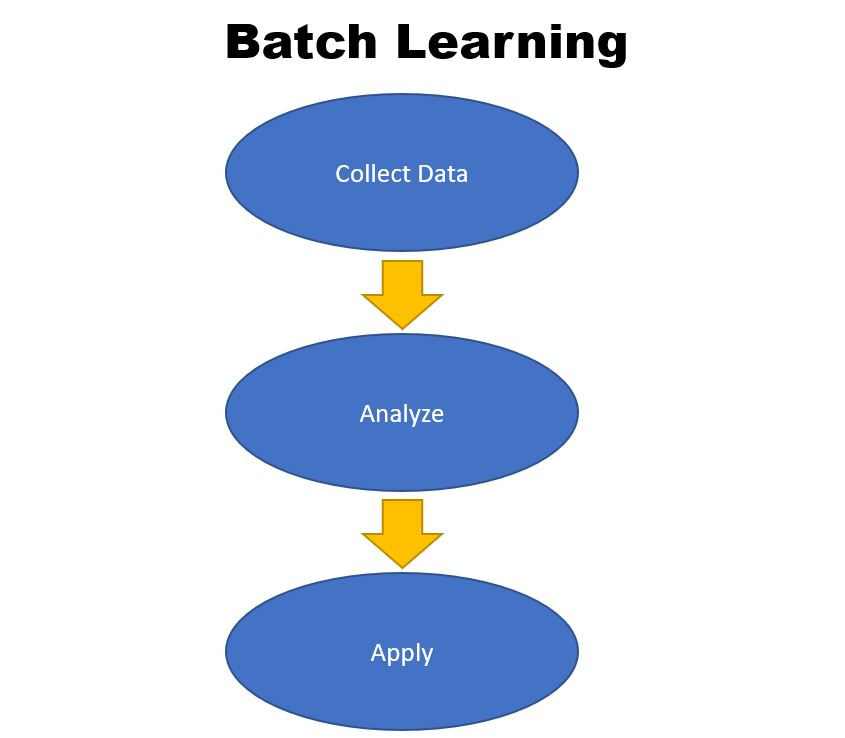
\includegraphics[width=0.99\linewidth]{figure/batch_learning}
			\end{figure}
			%	
		\end{minipage}
		%	
		\lz
		  \item The learning task on the available data beforehand is called the \emph{training phase} and the prediction on the unseen data is called the \emph{testing phase.} Both phases are \textbf{separated}.
		%	
	\end{itemize}
	%    
\end{frame}

\begin{frame}[t]
	\frametitle{Online learning}
%	
\begin{itemize} \small
%	
  	\item However, many real-world problems are \emph{dynamic} with the following aspects:
	%
	\lz
	
	\begin{minipage}{.6\textwidth}
	\begin{itemize} \small
		%	
		\item \emph{Sequential order ---} data is generated only bit by bit;
		%	
		\item \emph{On-the-fly decisions ---} decisions or predictions have to be made during the data generating process;
		%	
		\item \emph{Unforeseeable consequences ---} decisions can have a drastic influence on the data generating process;
		%	
		\item \emph{Constraints ---} there is a specific time limit or computational limit for the decision.
		%
	\end{itemize}
	\end{minipage}
	\begin{minipage}{.3\textwidth}
		\begin{figure}
		\centering
		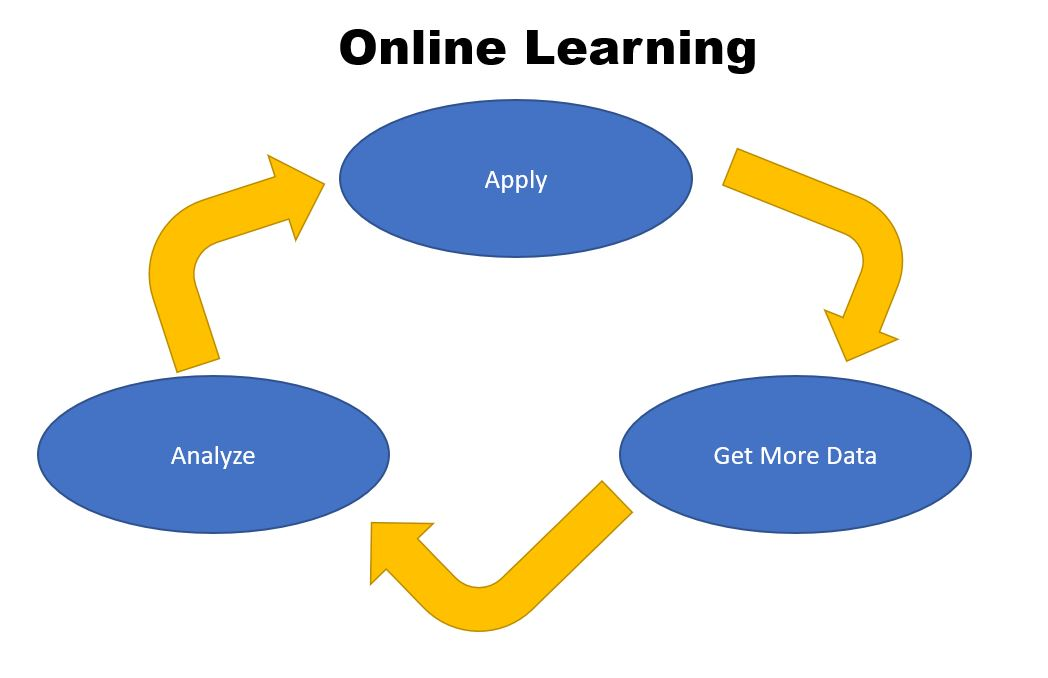
\includegraphics[width=0.99\linewidth]{figure/online_learning}
		\end{figure}
	%	
	\end{minipage}
	%
	\lz
	{\visible<2-> {	\item These dynamic aspects outline the framework where \textbf{online learning} is settled. 
	%
	\item Characteristically: In the online learning scenario the training phase and the testing phase are \textbf{interleaved}.}}
	%	
	%		
	\end{itemize}
%	
\end{frame}


\begin{frame}
	\frametitle{Online learning: Examples}
	%	
	\small
	There are many real-world applications which fit into the online learning scenario:
	%
	\begin{itemize} \small
		%
		  \item \emph{Weather Forecasting ---} Observe meteorological data as data streams by satellites for instance and keep the current weather prediction up to date.
		%	 
		%
		  \item \emph{Sequential Investment ---} A bank has to allocate its total capital on the financial market, where asset prices are varying over time.
		%
		%	 
		  \item \emph{Navigation systems ---} Find the best path from a to b given the current traffic situation.
		%
		%	 
		  \item \emph{Autonomous driving systems ---} Steer the automotive, while constantly monitoring the environment and react appropriately to any changes.
		%
		  \item $\ldots$
%		  
	\end{itemize}
	%
\end{frame}


\begin{frame}
\frametitle{Online learning: Illustration}
\small
%	
{\visible<1-> The data is available only in a \textbf{sequential order} generated by the environment and the learner's actions/predictions have to be made \textbf{on-the-fly.}}
%

{\visible<2-> {$\Rightarrow $ Learning algorithms have to be dynamically adapted (Update of the internal model).\\~} }
 
{\only<1>{
\begin{figure}
	\centering
	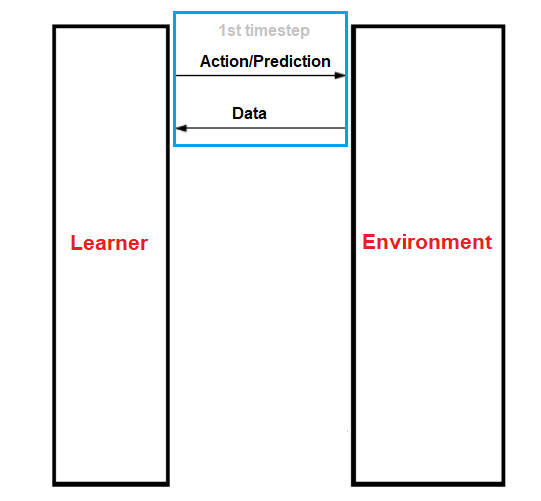
\includegraphics[width=0.4\linewidth]{figure/online_step_1}
\end{figure}}}
{\only<2>{
		\begin{figure}
			\centering
			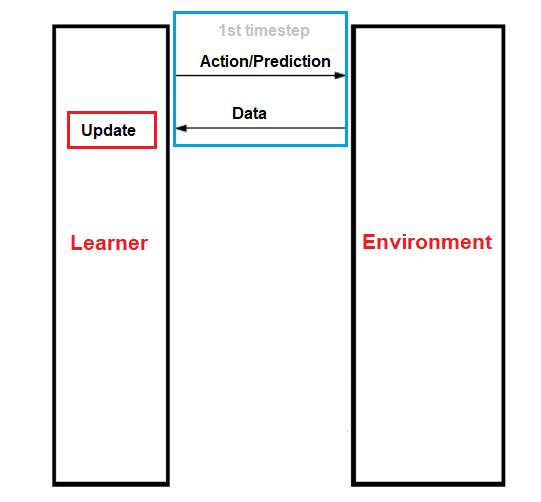
\includegraphics[width=0.4\linewidth]{figure/online_step_1_5}
\end{figure}}}
{\only<3>{
		\begin{figure}
			\centering
			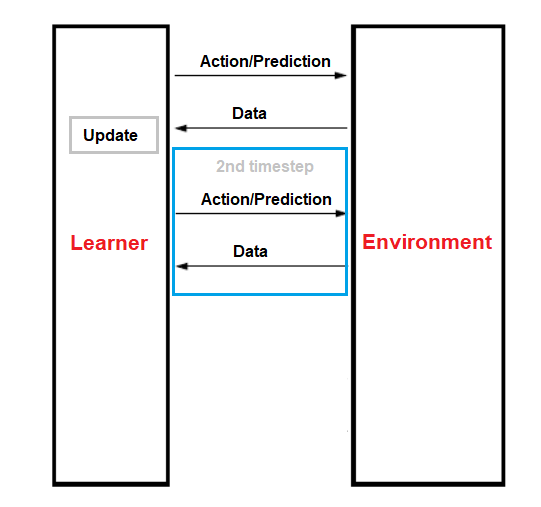
\includegraphics[width=0.4\linewidth]{figure/online_step_2}
\end{figure}}}
{\only<4>{
		\begin{figure}
			\centering
			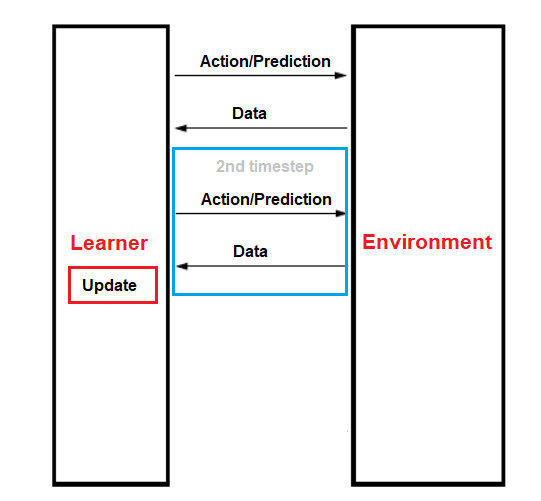
\includegraphics[width=0.4\linewidth]{figure/online_step_2_5}
\end{figure}}}
{\only<5>{
		\begin{figure}
			\centering
			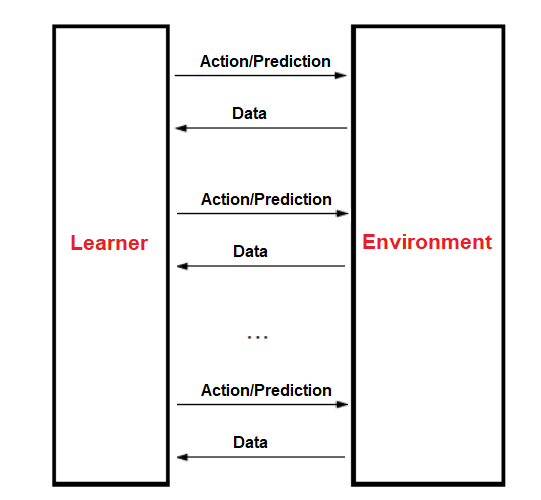
\includegraphics[width=0.4\linewidth]{figure/online_step_3}
\end{figure}}}


{\only<5>{$\Rightarrow $  The learner and the environment are alternately performing their actions.}}

\end{frame}




\begin{frame}{The basic online learning protocol}
	%	
	\footnotesize
	%	
	Formally, an online learning problem consists of:
	%
	\begin{itemize}\footnotesize
		%
		 \item a learner (forecaster, agent resp.\ decision maker), an environment (user resp.\ adversary, system resp.\ nature, ),
		%	
		 \item time steps $1,2,\ldots,T$ (may be infinite),
		%	
		 \item available actions $\mathcal A$ for the learner (may be infinite),
		%
		 \item environmental data space $\mathcal Z,$
		%
		 \item a loss function $\l: \mathcal{A} \times \mathcal{Z} \to \R.$
	\end{itemize}
	%
	{\visible<2-> {\textbf{Mechanism:} In each time step $t$
	%
	\begin{itemize}\footnotesize
		%
		 \item learner chooses an action $a_{t} \in \mathcal{A},$
		%
		 \item environment generates data $z_{t} \in \mathcal{Z},$
		%
		 \item learner observes the environmental data and suffers loss $\l(a_{t},z_{t}),$ 
		%	
		 \item learner update its model/ knowledge basis.
		%	
	\end{itemize}}}
	%
	{\visible<3-> {	Typically $\mathcal{A} = \mathcal{Z} = \Yspace$, so that
	%
	%
	\begin{itemize}\footnotesize
		%
		\item the learner's chosen action $a_{t} = \hat{y}_t$ corresponds to a prediction,
		%
		\item the generated data point $z_{t} =y_t$ is the revealed outcome.
		%	
	\end{itemize}}}
\end{frame}

\begin{frame}{The extended online learning protocol}
	%	
\footnotesize
\begin{itemize}
	%		
	 \item In some applications, the environmental data consists of two parts: $z_{t} = (z_{t}^{(1)}, z_{t}^{(2)}),$ where the first part of the data, $z_{t}^{(1)},$ is revealed to the learner \textbf{before} the action is made.
	%
	After the learner carries out its action, the remaining part of the environmental data is revealed, that is, $z_{t}^{(2)}.$
	%
	{\visible<2-> {  \item The \textbf{mechanism} in such an online learning problem is then as follows: In each time step $t$
	%
	\begin{itemize}\footnotesize
		%
		 \item the environment generates data $z_{t} = (z_{t}^{(1)}, z_{t}^{(2)}) \in \mathcal{Z},$
		%	
		 \item the learner observes the first part of the environmental data $ z_{t}^{(1)},$
		%	
		 \item the learner chooses an action $a_{t} \in \mathcal{A},$  
		%
		 \item the learner observes the remaining part of the environmental data $z_{t}^{(2)}$ and suffers loss $\l(a_{t},z_{t}),$ 
		%	
		 \item the learner updates its knowledge base.
		%	
	\end{itemize} }}
	%
	{\visible<3-> {  \item Apparently, the learner can  take the a priori information in form of $ z_{t}^{(1)}$ at each time step $t$ into account when choosing its action. }}
	% 
	%
	{\visible<4-> {  \item We call this setting the \emph{extended online learning protocol.}	}}
%	 
	 {\visible<5-> { \item 	Typically $\mathcal{A} = \Yspace$ and  $ \mathcal{Z} = \Xspace \times \Yspace$, so that
	 		%
	 		%
	 		\begin{itemize}\footnotesize
	 			%
	 			\item the first part $z_{t}^{(1)} = \xv_t$ is some feature information,
	 			%	
	 			\item the learner's chosen action $a_{t} = \hat{y}_t$ corresponds to a prediction (dep.\ on $\xv_t$),
%	 			
				\item the second part $z_{t}^{(2)} =y_t$ is the corresponding outcome.
%	 			
	 \end{itemize}}}	
\end{itemize}
%
\end{frame}


\begin{frame}{Data generation in Online learning}
%	
	\begin{itemize}
%		
		\item Typically for the online learning setting is that \textbf{no} statistical assumptions is made on how the sequence of environmental data is generated.
%		
		\item In particular, the environmental data are not necessarily generated by a probability distribution!
%		
		\item This also covers the area of \emph{adversarial learning}: the data can even be generated by an adversary trying to fool the learner.
%		
		\item However, the online learning setting can of course also be considered in a statistical setting.
%		
	\end{itemize}
%	
\end{frame}


\begin{frame}{Online learning: Requirements}
	%
	\small
	\begin{itemize}
		%	
		\item The dynamical aspects have to be incorporated for the design of efficient learning algorithms. 
		%	
		 \item The online learner has to cope with the sequential availability of the data and to cope with time as well as computational constraints.
		%	
		 \item Roughly speaking, one seeks to construct an online learning algorithm which is adaptive to the environment and allows incremental as well as preferably cheap updates over time.
		%	
		 \item Although consideration of time and memory constraints is important for practical purposes, we will only implicitly consider these constraints in this lecture. 
		%	
		 \item We will mainly focus our theoretical analysis on the performance of the learner in terms of its (cumulative) loss, which, however, will usually ignore computational aspects of the learner.
		%
	\end{itemize}
	%
\end{frame}


\begin{frame} 
	{Regret in Online learning: Measure of Quality}
	%
	\footnotesize
	%
	\begin{itemize}
		%	
		\item In order to measure the quality of an online learner one can compute the difference between the cumulative loss of the learner and the cumulative loss by taking some competing action $a\in \A:$
		%
		\begin{align*}
			%	 \label{defi_regret_competing}
			%	
			R_T(a) = \sum\nolimits_{t=1}^T \l(a_{t},z_{t}) - \sum\nolimits_{t=1}^T \l(a, z_{t}).
			%	
		\end{align*}
		%
		 \item This value is called the \emph{(cumulative) regret of a learner} with respect to an action $a \in \A.$
		%
		 \item {\visible<2->{  It seems natural to compare the incurred cumulative loss of the learner with the \emph{best action(s) in hindsight}:
		%
		\begin{align*}
			%	 \label{defi_regret}
			%	
			R_T = \sum\nolimits_{t=1}^T \l(a_{t},z_{t}) - \inf_{a\in \A} \sum\nolimits_{t=1}^T \l(a, z_{t}).
			%	
		\end{align*} 
		%
		 \item Here, 
%		 
		 \begin{itemize} \footnotesize
			%		
			 \item  $\sum_{t=1}^T \l(a_{t},z_{t})$ is the \emph{cumulative loss of the learner},
			%		
			 \item $\inf_{a\in \A} \sum_{t=1}^T \l(a, z_{t})$ is the cumulative loss of the \emph{best action(s) in hindsight}. 
		\end{itemize} }}
		%
		 \item {\visible<3>{  We refer to $R_T$ as the \emph{(cumulative) regret} of the online learner. It is easy to see that $R_T = \sup_{a\in \A} R_T(a).$ }}
		%
	\end{itemize}
	%
\end{frame}
%	
\begin{frame} 
	{Regret in Online learning: Measure of Quality}
	%
	\small
	\begin{itemize}
		\item The objective of the online learner is to minimize the cumulative regret $R_T.$
		%	
		 \item {\visible<2->{  Note that the cumulative regret can be in principle negative as the action sequence could be such that $\l(a_{s},z_{s}) <    \l(a^*,z_{s})$ holds for specific time steps $s,$ where $a^* \in \argmin_{a \in \A } \sum_{s=1}^T \l(a,z_{s})$ is one of the best actions in hindsight (may be unique). }}
		%	
		%	If this is possible (which will be rarely the case), then the goal of the learner is to achieve the lowest cumulative regret possible.
		%
		 \item {\visible<3->{  If the cumulative regret is always non-negative (which will be usually the case), then the overall goal of an online learner is to have a regret which is \emph{sublinear} in the time horizon $T.$ }}
		%	
		{\visible<4>{  \item Formally, the following should hold 
		%
		\begin{align*}
				R_T	= o(T).	
		\end{align*}
		%
		\emph{Interpretation:} The average regret per time step (or per example) goes to zero: 
		%	
		\begin{align*}
			  \frac1T \Big( \sum_{t=1}^T \l(a_{t},z_{t}) - \inf_{a\in \A} \sum_{t=1}^T \l(a, z_{t}) \Big) = \frac{R_T}{T} = o(1).
		\end{align*} }}
		%
	\end{itemize}
	%
\end{frame}


\begin{frame}
	{Dynamic regret}
%	
	\begin{itemize}
%		
		\item One might ask why one compares only with a fixed best action in hindsight, say $a^*$, instead of a sequence of actions $a_1^*,a_2^*,\ldots,a_T^*?$ 
		%	
		{\visible<2->{  \item The rationale behind this measure of quality is that the best	fixed action in hindsight is already reasonably good over all the time steps: it performs almost as well as a batch learner that
		observes the entire sequence and picks the best action in hindsight. }}
		%	
		{\visible<3->{  \item However, this is too optimistic and may not hold in changing environments, where data are evolving and the optimal action is drifting over the time. }}
		%	
		{\visible<4->{  \item To address this limitation, recent works have also considered the \emph{dynamic regret}:
		%	
		\begin{align*}
			%	 \label{defi_dynamic_regret}
			%	
			R_T^D(a_1^*,a_2^*,\ldots,a_T^*) = \sum\nolimits_{t=1}^T \l(a_{t},z_{t}) -   \sum\nolimits_{t=1}^T \l(a_t^*, z_{t}).
			%	
		\end{align*} }}
%	
		{\visible<5->{  \item We will cover only the static regret in this lecture.}}
%		
	\end{itemize}
%	
\end{frame}



%
\endlecture
\end{document}
